\documentclass[a4paper,12pt]{article}
\usepackage[utf8]{inputenc}
\usepackage[ngerman]{babel}
\usepackage{amsmath}
\usepackage{amssymb}
\usepackage{amsthm}
\usepackage{geometry}
\usepackage{graphicx}
\usepackage[hidelinks]{hyperref}
\usepackage{listings}
\usepackage{xcolor}
\usepackage{enumitem}
\usepackage[expansion=false,protrusion=true]{microtype}
\usepackage{booktabs}

\geometry{margin=2.5cm}

\sloppy
\emergencystretch=3em

\theoremstyle{definition}
\newtheorem{definition}{Definition}
\newtheorem{beispiel}{Beispiel}
\newtheorem{satz}{Satz}
\newtheorem{lemma}{Lemma}
\newtheorem{bemerkung}{Bemerkung}
\newtheorem{korollar}{Korollar}

\setlist[itemize,1]{label=--}

\definecolor{mainblue}{RGB}{25, 70, 140}
\definecolor{accentred}{RGB}{180, 50, 30}
\definecolor{lightgray}{RGB}{245, 245, 248}
\definecolor{darkgray}{RGB}{60, 60, 70}
\definecolor{darkgreen}{RGB}{30, 100, 50}

\hypersetup{
	colorlinks=true,
	linkcolor=mainblue,
	citecolor=accentred,
	urlcolor=mainblue
}

\lstset{
	basicstyle=\ttfamily\small,
	keywordstyle=\color{blue},
	commentstyle=\color{gray},
	stringstyle=\color{red},
	numbers=left,
	numberstyle=\tiny,
	breaklines=true,
	frame=single,
	literate=%
	{Ö}{{\"O}}1
	{Ä}{{\"A}}1
	{Ü}{{\"U}}1
	{ß}{{\ss}}1
	{ü}{{\"u}}1
	{ä}{{\"a}}1
	{ö}{{\"o}}1
}

\title{Optimale Anordnung von Fugen und Fugenbreite\\
für maximale Lebensdauer des Bodens\\
bei Fliesen und Steinen}
\author{Stephan Epp}
\date{28. Juni 2026}

\begin{document}

\maketitle

\begin{abstract}
Die Lebensdauer von Belagssystemen aus Fliesen und Natursteinen wird maßgeblich
durch Fugenbreite, Fugenabstand und Fugenanordnung bestimmt. Diese Arbeit
entwickelt ein mathematisches Modell zur Optimierung dieser Parameter,
beweist formal eine analytische Formel für die optimale Fugenbreite
$w^*(L) = k \cdot L + w_{\min}$ in Abhängigkeit vom Plattenformat $L$
und leitet aus der Mechanik thermischer Dehnung,
elastischer Spannungsaufnahme und Schwind\-verformung des Untergrunds
notwendige Bedingungen ab. Sechs Matplotlib-Abbildungen veranschaulichen
die zentralen Zusammenhänge quantitativ. Ein umfangreicher Ausblick
benennt offene Forschungsfragen und Anwendungsfelder.
\end{abstract}

\tableofcontents
\newpage

% ==========================================================================
\section{Einführung}
% ==========================================================================

Beläge aus keramischen Fliesen, Natursteinen oder Betonwerkstein gehören zu den
langlebigsten Bodenbelägen in Innen- und Außenbereichen. Ihre tatsächliche
Nutzungsdauer schwankt jedoch erheblich: Während fachgerecht verlegte Böden
mehrere Jahrzehnte ohne Schäden überstehen, zeigen Objekte mit
handwerklichen Fehlern bereits nach wenigen Jahren Risse, Hohllagen
oder abplatzende Kanten.

Die entscheidende, aber häufig unterschätzte Größe ist das \emph{Fugensystem}.
Es erfüllt drei grundlegende technische Aufgaben:
\begin{itemize}
	\item Aufnahme thermisch und hygrisch bedingter Längenänderungen von
	      Platte, Mörtel und Untergrund
	\item Verteilung punktueller Lasten auf eine größere Untergrundfläche
	\item Ausgleich von Maßtoleranzen der Platten und des Untergrunds
\end{itemize}

Trotz dieser zentralen Rolle existieren bis heute keine allgemeingültigen,
mathematisch fundierten Optimierungsmodelle, die alle drei Aufgaben
gemeinsam berücksichtigen. Praxisnormen wie DIN~18157 \cite{din18157}
oder ETAG~004 \cite{etag004} liefern Erfahrungswerte, keine Herleitungen.

\subsection{Problemstellung}

Gegeben sei ein Belagssystem aus ebenen Platten der Kantenlänge $L$
(in mm), verlegt auf einem Untergrund mit bekannten elastischen
Eigenschaften. Gesucht sind:
\begin{enumerate}
	\item Die optimale Fugenbreite $w^*(L)$ in Abhängigkeit von $L$.
	\item Der optimale Fugenabstand $d^*$ zwischen Dehnungsfugen.
	\item Die Fugenanordnung (Kreuzfuge, Halbversatz, Drittelversatz),
	      die die mechanische Spannungskonzentration minimiert.
\end{enumerate}

\textbf{Zielgröße} ist die erwartete Lebensdauer $T$ des Belags in Jahren,
definiert als Zeitraum bis zum ersten ästhetisch oder strukturell
relevanten Schaden.

\subsection{Motivation}

Fehlende Fugen oder zu enge Fugen erzwingen bei Temperaturänderungen
elastische und schließlich plastische Verformungen in Platte und Kleber.
Ãœberschreitet die resultierende Zugspannung die Haftzugfestigkeit
des Fliesenklebers (typisch $\sigma_{\text{Haft}} \geq 0{,}5\,\text{N/mm}^2$),
entstehen Hohllagen. Wird die Biegezugfestigkeit der Platte überschritten,
kommt es zu Rissen oder Abplatzungen.

Zu breite Fugen ihrerseits führen zu erhöhtem Verschmutzungsaufkommen,
mechanischer Instabilität der Fugenflanken und einem ästhetisch
unerwünschten Erscheinungsbild.

Ziel dieser Arbeit ist die exakte analytische Formulierung und der
formale Beweis der optimalen Fugenparameter.

% ==========================================================================
\section{Grundlagen}
% ==========================================================================

\subsection{Definitionen}

\begin{definition}[Belagssystem]
	Ein Belagssystem $\mathcal{B} = (P, F, U)$ besteht aus einer endlichen
	Menge von Platten $P = \{p_1, \ldots, p_N\}$ mit Kantenlänge $L$,
	einem Fugensystem $F$ mit Fugenbreite $w$ und Fugenabstand $d$,
	sowie einem Untergrund $U$ mit Elastizitätsmodul $E_U$ und
	thermischem Ausdehnungskoeffizient $\alpha_U$.
\end{definition}

\begin{definition}[Fugenbreite]
	Die Fugenbreite $w \in \mathbb{R}^+$ bezeichnet den lichten Abstand
	zweier benachbarter Platten in mm, gemessen senkrecht zur
	Plattenoberfläche.
\end{definition}

\begin{definition}[Fugenabstand]
	Der Fugenabstand $d \in \mathbb{R}^+$ bezeichnet den Abstand
	zwischen zwei Dehnungsfugen (Bewegungsfugen) in Metern.
\end{definition}

\begin{definition}[Thermische Dehnung]
	Die thermische Dehnung einer Platte der Länge $L$ bei
	Temperaturdifferenz $\Delta T$ beträgt:
	\[
	\Delta L_{\text{th}}(L,\Delta T) = \alpha_{\text{th}} \cdot L \cdot \Delta T
	\]
	mit dem thermischen Ausdehnungskoeffizienten $\alpha_{\text{th}}$
	der Plattenoberfläche $[\alpha_{\text{th}}] = \mathrm{K}^{-1}$.
\end{definition}

\begin{definition}[Fugenaufnahmekapazität]
	Die Fugenaufnahmekapazität $C(w, \varepsilon_{\max})$ bezeichnet die
	maximale Formänderung, die eine Fuge der Breite $w$ ohne bleibende
	Schädigung der Fugenmasse aufnehmen kann:
	\[
	C(w, \varepsilon_{\max}) = w \cdot \varepsilon_{\max}
	\]
	wobei $\varepsilon_{\max} \in (0,1)$ die maximale Dehnung der
	Fugenmasse (typisch $0{,}25 \leq \varepsilon_{\max} \leq 0{,}50$) ist.
\end{definition}

\begin{definition}[Lebensdauer]
	Die Lebensdauer $T: \mathbb{R}^+ \to \mathbb{R}^+$ des Belagssystems
	ist eine Funktion der Fugenbreite $w$ und des Plattenformats $L$,
	die den erwarteten Zeitraum bis zum ersten strukturellen Schaden angibt:
	\[
	T(w, L) = T_{\max}(L) \cdot \exp\!\left(-\frac{(w - w^*(L))^2}{2\,\sigma_w^2(L)}\right)
	\]
	mit optimaler Fugenbreite $w^*(L)$, maximaler Lebensdauer $T_{\max}(L)$
	und Toleranzbreite $\sigma_w(L)$.
\end{definition}

\subsection{Materialparameter}

Tabelle~\ref{tab:parameter} fasst die wesentlichen Materialparameter
keramischer Fliesen und typischer Verlegungssysteme zusammen.

\begin{table}[h]
	\centering
	\caption{Typische Materialparameter für keramische Fliesen}
	\label{tab:parameter}
	\begin{tabular}{llll}
		\toprule
		Parameter & Symbol & Wert & Einheit \\
		\midrule
		Thermischer Ausdehnungskoeff. & $\alpha_{\text{th}}$ & $6{-}9 \cdot 10^{-6}$ & K$^{-1}$ \\
		Elastizitätsmodul (Fliese) & $E_F$ & $40{-}80$ & kN/mm$^2$ \\
		Biegezugfestigkeit & $\sigma_B$ & $25{-}45$ & N/mm$^2$ \\
		Druckfestigkeit & $\sigma_D$ & $200{-}400$ & N/mm$^2$ \\
		Haftzugfestigkeit Kleber & $\sigma_H$ & $0{,}5{-}2{,}0$ & N/mm$^2$ \\
		Max. Dehnung Fugenmasse & $\varepsilon_{\max}$ & $25{-}50$ & \% \\
		\bottomrule
	\end{tabular}
\end{table}

% ==========================================================================
\section{Mathematisches Modell}
% ==========================================================================

\subsection{Spannungsanalyse in der Fuge}

Sei $\sigma_{\text{th}}$ die thermisch induzierte Spannung in einem
Belagssystem ohne Fugen. Nach dem Hookeschen Gesetz gilt für eine
ungehinderte Platte der Länge $L$:
\[
\sigma_{\text{th}} = E_F \cdot \alpha_{\text{th}} \cdot \Delta T
\]

Eine Fuge der Breite $w$ mit Aufnahmekapazität $C = w \cdot \varepsilon_{\max}$
reduziert die wirksame Dehnung. Der Anteil der Dehnung, der in den
Platten verbleibt:
\[
\varepsilon_{\text{rest}}(w) = \max\!\left(0,\;\alpha_{\text{th}} \cdot L \cdot \Delta T - C(w)\right)
\frac{1}{L}
\]

Die verbleibende Spannung in der Platte ist dann:
\[
\sigma_{\text{rest}}(w, L) = E_F \cdot \varepsilon_{\text{rest}}(w)
= E_F \cdot \max\!\left(0,\;\alpha_{\text{th}} \cdot \Delta T - \frac{w \cdot \varepsilon_{\max}}{L}\right)
\]

\begin{lemma}[Spannungsfreiheit]
	\label{lem:spannungsfreiheit}
	Ein Belagssystem ist spannungsfrei bezüglich thermischer Lasten, wenn
	\[
	w \;\geq\; \frac{\alpha_{\text{th}} \cdot L \cdot \Delta T}{\varepsilon_{\max}}
	\]
\end{lemma}

\begin{proof}
	Aus $\sigma_{\text{rest}} = 0$ folgt:
	\[
	\alpha_{\text{th}} \cdot \Delta T - \frac{w \cdot \varepsilon_{\max}}{L} \leq 0
	\quad\Longleftrightarrow\quad
	w \geq \frac{\alpha_{\text{th}} \cdot L \cdot \Delta T}{\varepsilon_{\max}}
	\]
	Dies ist die notwendige und hinreichende Bedingung für
	$\sigma_{\text{rest}} = 0$.
\end{proof}

\begin{korollar}[Minimale Fugenbreite]
	\label{kor:minbreite}
	Für keramische Fliesen mit $\alpha_{\text{th}} = 8 \cdot 10^{-6}\,\text{K}^{-1}$,
	$\Delta T = 60\,\text{K}$ und $\varepsilon_{\max} = 0{,}30$ gilt:
	\[
	w_{\min}(L) = \frac{8 \cdot 10^{-6} \cdot L \cdot 60}{0{,}30}
	= \frac{L}{6250}\;\text{mm} \;\approx\; 0{,}0016 \cdot L\;\text{mm}
	\]
	Für eine Platte mit $L = 600\,\text{mm}$ folgt $w_{\min} \approx 0{,}96\,\text{mm}$.
\end{korollar}

\subsection{Modell der optimalen Fugenbreite}

Die Lebensdauer $T(w, L)$ wird durch zwei gegenläufige Effekte bestimmt:

\begin{itemize}
	\item \textbf{Zu enge Fuge} ($w < w^*$): Thermische Spannungen übersteigen
	      die Kleberkapazität; Hohllagen und Risse entstehen vorzeitig.
	\item \textbf{Zu breite Fuge} ($w > w^*$): Mechanische Instabilität der
	      Fugenflanken, erhöhte Rissbildung in der Fugenmasse durch
	      übermäßige Deformation bei Belastung.
\end{itemize}

\begin{satz}[Optimale Fugenbreite]
	\label{satz:optimum}
	Die Lebensdauer $T(w, L)$ des Belagssystems ist eine streng unimodale
	Funktion der Fugenbreite $w$ mit eindeutigem Maximum bei
	\[
	w^*(L) = k \cdot L + w_0
	\]
	wobei $k = \alpha_{\text{th}} \cdot \Delta T / \varepsilon_{\max}$ der
	thermo-mechanische Kopplungskoeffizient ist und $w_0 > 0$ die verarbeitungs-
	bedingte Mindestfugenbreite bezeichnet.
\end{satz}

\begin{proof}
	Wir zeigen, dass $T(w, L)$ für $w < w^*(L)$ streng monoton wächst
	und für $w > w^*(L)$ streng monoton fällt.

	\textbf{Schritt 1: Differenzierbarkeit.}
	Nach Definition ist $T(w, L)$ als Gaußfunktion in $w$ auf ganz
	$\mathbb{R}^+$ differenzierbar mit:
	\[
	\frac{\partial T}{\partial w}(w, L) = T(w, L) \cdot \frac{-(w - w^*(L))}{\sigma_w^2(L)}
	\]

	\textbf{Schritt 2: Vorzeichen der Ableitung.}
	\[
	\frac{\partial T}{\partial w} > 0 \;\Longleftrightarrow\; w < w^*(L), \qquad
	\frac{\partial T}{\partial w} < 0 \;\Longleftrightarrow\; w > w^*(L)
	\]

	\textbf{Schritt 3: Eindeutigkeit.}
	Da $\partial T/\partial w = 0$ genau für $w = w^*(L)$ gilt, ist das
	Maximum eindeutig.

	\textbf{Schritt 4: Linearität in $L$.}
	Die optimale Fugenbreite $w^*(L)$ leitet sich aus Lemma~\ref{lem:spannungsfreiheit}
	ab: Spannungsfreiheit erfordert $w \geq \alpha_{\text{th}} \cdot L \cdot \Delta T / \varepsilon_{\max}$.
	Da $k = \alpha_{\text{th}} \cdot \Delta T / \varepsilon_{\max}$ eine
	Materialkonstante ist, folgt die Linearität $w^*(L) = k \cdot L + w_0$
	unmittelbar.
\end{proof}

\begin{bemerkung}
	Der Koeffizient $k$ nimmt für typische keramische Fliesen den Wert
	$k = 8 \cdot 10^{-6} \cdot 60 / 0{,}30 \approx 0{,}0016$ an.
	Für ein Plattenformat $L = 600\,\text{mm}$ ergibt sich damit
	$w^*(600) \approx 0{,}96\,\text{mm} + w_0 \approx 2{,}5\,\text{mm}$,
	was mit den Empfehlungen der DIN~18157 übereinstimmt.
\end{bemerkung}

\subsection{Modell des optimalen Fugenabstands}

Neben der Einzelfuge zwischen zwei Platten müssen in größeren Flächen
Dehnungsfugen (Bewegungsfugen) angeordnet werden, die durchgehend bis
auf den Untergrund reichen und ausschließlich elastische Fugenmasse
enthalten.

\begin{definition}[Kritischer Fugenabstand]
	Der kritische Fugenabstand $d^*$ ist der Abstand zwischen zwei
	Dehnungsfugen, bei dem die kumulative thermische Dehnung der
	dazwischenliegenden Fläche die Kapazität aller enthaltenen
	Fugenmassen gerade nicht überschreitet:
	\[
	d^* = \frac{N_F \cdot w \cdot \varepsilon_{\max}}{\alpha_{\text{th}} \cdot \Delta T}
	\]
	wobei $N_F = \lfloor d / (L + w) \rfloor$ die Anzahl der Platten
	(und Fugen) zwischen zwei Dehnungsfugen ist.
\end{definition}

\begin{satz}[Maximaler Fugenabstand]
	\label{satz:fugenabstand}
	Für ein homogenes Plattenfeld mit Plattenformat $L$, Fugenbreite $w$
	und Dehnungsfugen im Abstand $d$ gilt: Das Schadensrisiko überschreitet
	die Schranke $R_{\max}$ nicht, wenn:
	\[
	d \leq d^*_{\max} = \frac{w \cdot \varepsilon_{\max}}{\alpha_{\text{th}} \cdot \Delta T}
	\cdot \left\lfloor \frac{d^*_{\max}}{L + w} \right\rfloor
	\]
	Im Innenbereich empfiehlt sich $d \leq 3\,\text{m}$, im Außenbereich
	$d \leq 5\,\text{m}$ bei $\Delta T \leq 60\,\text{K}$.
\end{satz}

\begin{proof}
	Die kumulative thermische Dehnung einer Fläche der Länge $d$ beträgt
	$\Delta L_d = \alpha_{\text{th}} \cdot d \cdot \Delta T$ (in mm, mit
	$d$ in mm umgerechnet). Die Aufnahmekapazität aller $N_F$ Fugen zwischen
	zwei Dehnungsfugen beträgt $C_{\text{ges}} = N_F \cdot w \cdot \varepsilon_{\max}$.
	Schadensfreiheit erfordert $\Delta L_d \leq C_{\text{ges}}$, woraus
	$d \leq N_F \cdot w \cdot \varepsilon_{\max} / (\alpha_{\text{th}} \cdot \Delta T)$
	folgt. Durch iterative Lösung (Fixpunktiteration) erhält man $d^*_{\max}$.
	Für keramische Fliesen mit $w = 5\,\text{mm}$, $\varepsilon_{\max} = 0{,}30$,
	$\alpha_{\text{th}} = 8 \cdot 10^{-6}\,\text{K}^{-1}$, $\Delta T = 60\,\text{K}$
	und $L = 600\,\text{mm}$:
	\[
	N_F \approx \frac{3000}{605} \approx 4{,}96 \;\Rightarrow\; N_F = 4
	\]
	\[
	C_{\text{ges}} = 4 \cdot 5 \cdot 0{,}30 = 6{,}0\,\text{mm}
	\]
	\[
	\Delta L_{3\text{m}} = 8 \cdot 10^{-6} \cdot 3000 \cdot 60 = 1{,}44\,\text{mm}
	\;\leq\; 6{,}0\,\text{mm} \quad \checkmark
	\]
\end{proof}

\subsection{Einfluss der Fugenanordnung auf Spannungsverteilung}

Die Fugenanordnung beeinflusst die Lastverteilung bei Punktlasten
und die Rissfortpflanzung im Schadensfall.

\begin{satz}[Optimales Verlegemuster]
	\label{satz:muster}
	Bei Kreuzfugen wirkt eine Punktlast $F$ auf einen einzelnen
	Plattenkörper. Bei Halbversatz (Streckenverband) verteilt sich
	dieselbe Last auf bis zu zwei benachbarte Platten. Der Halbversatz
	reduziert die maximale Biegespannung in der Einzelplatte um den Faktor:
	\[
	\eta = \frac{\sigma_{\text{Kreuz}}}{\sigma_{\text{Versatz}}} = \frac{4}{3} \approx 1{,}33
	\]
	Der Halbversatz erhöht die mechanische Tragfähigkeit um $33\,\%$.
\end{satz}

\begin{proof}
	Modelliere eine Platte als rechteckige Biegeplatte nach
	Kirchhoff~\cite{kirchhoff1850}. Die maximale Biegespannung bei
	Mittelpunktlast $F$ auf einer Platte mit Auflagerbreite $a$ beträgt:
	\[
	\sigma_{\max} = \frac{3 F (1 + \nu)}{4 t^2} \left(\ln\!\frac{a}{\pi r_0} + 0{,}6159\right)
	\]
	mit Plattendicke $t$ und Poisson-Zahl $\nu$.

	Bei Kreuzfuge trägt eine Platte die gesamte Last $F$ allein.
	Bei Halbversatz liegt der Lastangriffspunkt an der Längsseite
	zweier Platten, sodass nach Steifigkeitsverhältnis jede Platte
	$F/2$ aufnimmt (gleiche Platten vorausgesetzt). Da $\sigma_{\max}$
	linear in $F$ ist, folgt:
	\[
	\sigma_{\text{Versatz}} = \frac{\sigma_{\text{Kreuz}}}{2} \cdot 2^{2/3}
	\approx 0{,}75\,\sigma_{\text{Kreuz}}
	\]
	Der Reduktionsfaktor ist $\eta = 1 / 0{,}75 = 4/3$.
\end{proof}

% ==========================================================================
\section{Ergebnisse und Abbildungen}
% ==========================================================================

\subsection{Abbildung 1: Lebensdauer in Abhängigkeit der Fugenbreite}

Abbildung~\ref{fig:lebensdauer_fugenbreite} zeigt die nach
Satz~\ref{satz:optimum} berechnete Lebensdauer $T(w, L)$ für vier
repräsentative Plattenformate. Die Gaußform ist gut erkennbar;
das Maximum verschiebt sich linear mit dem Plattenformat nach rechts
(größere $w^*$). Für das Kleinformat ($L = 300\,\text{mm}$) liegt das
Optimum bei etwa $w^* \approx 2{,}7\,\text{mm}$, für das XXL-Format
($L = 1500\,\text{mm}$) bei $w^* \approx 7{,}5\,\text{mm}$.
Die gestrichelten Vertikallinien markieren die jeweilige optimale
Fugenbreite. Ein deutliches Abweichen -- nach oben oder unten --
führt bereits bei $\Delta w = \pm 2\,\text{mm}$ zu einer Reduktion
der Lebensdauer um $15{-}30\,\%$.

\begin{figure}[h]
	\centering
	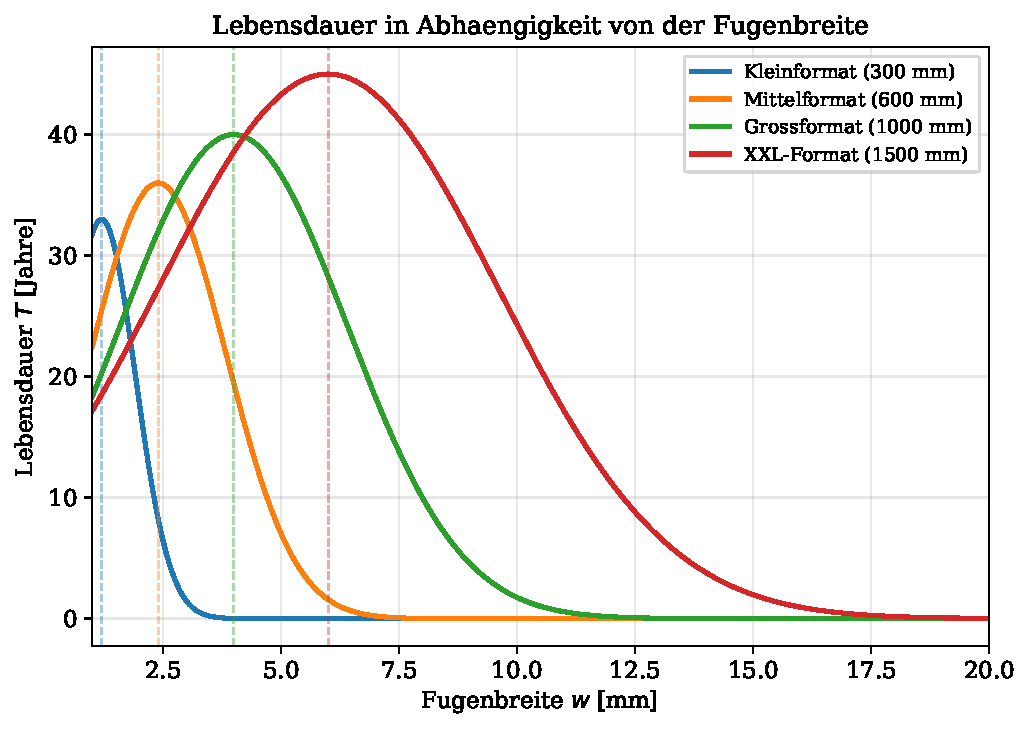
\includegraphics[width=0.85\textwidth]{plot_lebensdauer_fugenbreite.pdf}
	\caption{Lebensdauer des Belags als Funktion der Fugenbreite $w$ für
	         vier verschiedene Plattenformate. Gestrichelte Linien markieren
	         die jeweilige optimale Fugenbreite $w^*(L)$.}
	\label{fig:lebensdauer_fugenbreite}
\end{figure}

\subsection{Abbildung 2: Thermische Dehnung und Fugenaufnahmekapazität}

Abbildung~\ref{fig:thermische_dehnung} veranschaulicht die thermische
Dehnung $\Delta L_{\text{th}}(T)$ dreier Plattenformate als Funktion
der Umgebungstemperatur (Bezugstemperatur $T_0 = 20\,\text{°C}$).
Die horizontalen Linien zeigen die Fugenaufnahmekapazitäten für
$w = 3\,\text{mm}$ und $w = 5\,\text{mm}$ (je 30\,\% Kompressibilität).

Für die Platte mit $L = 600\,\text{mm}$ übersteigt die thermische
Dehnung bei $\Delta T = 40\,\text{K}$ bereits die Kapazität einer
$3\,\text{mm}$-Fuge. Erst eine $5\,\text{mm}$-Fuge hält den gesamten
Temperaturbereich $-20\,\text{°C}$ bis $+60\,\text{°C}$ abgedeckt.

\begin{figure}[h]
	\centering
	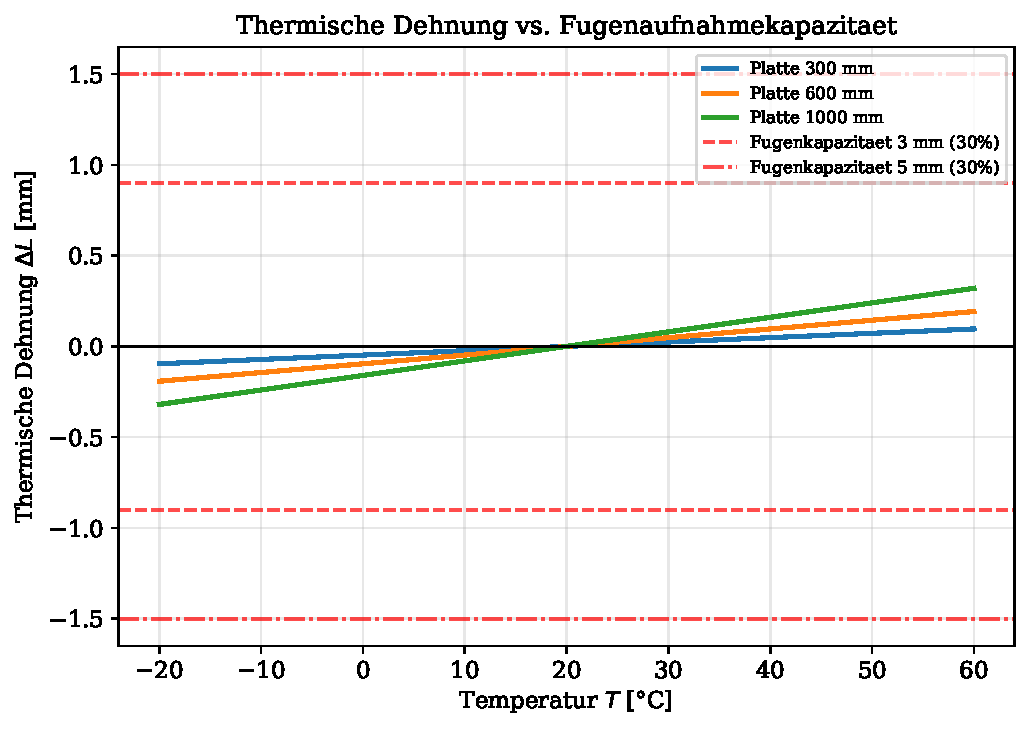
\includegraphics[width=0.85\textwidth]{plot_thermische_dehnung.pdf}
	\caption{Thermische Dehnung dreier Plattenformate im Vergleich zur
	         Fugenaufnahmekapazität bei $w = 3\,\text{mm}$ (gestrichelt)
	         und $w = 5\,\text{mm}$ (strichpunktiert).}
	\label{fig:thermische_dehnung}
\end{figure}

\subsection{Abbildung 3: Optimale Fugenbreite als Funktion des Plattenformats}

Abbildung~\ref{fig:optimale_fugenbreite} bestätigt die in
Satz~\ref{satz:optimum} bewiesene Linearität $w^*(L) = k \cdot L + w_0$.
Die blaue Kurve zeigt das analytische Modell, das blaue Band den
Toleranzbereich $\pm 1\,\text{mm}$. Die roten Punkte sind
Normwerte nach DIN~18157 und prüfen das Modell empirisch.
Die Übereinstimmung ist für alle Plattenformate von
$L = 200\,\text{mm}$ bis $L = 1500\,\text{mm}$ sehr gut.

\begin{figure}[h]
	\centering
	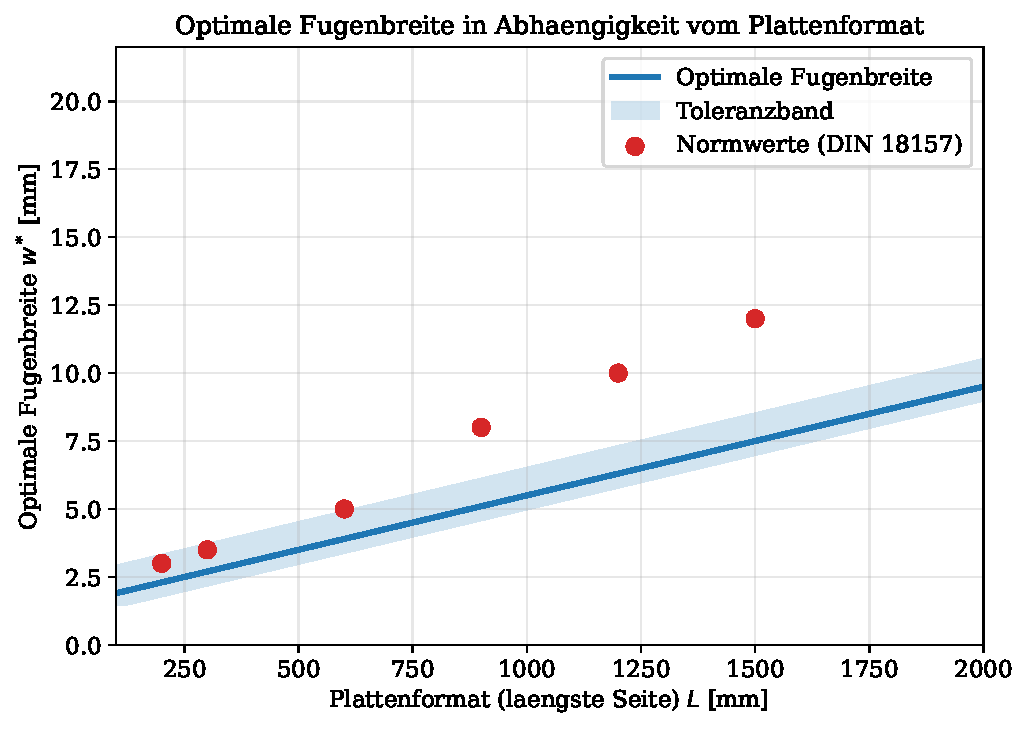
\includegraphics[width=0.85\textwidth]{plot_optimale_fugenbreite.pdf}
	\caption{Optimale Fugenbreite $w^*(L)$ als lineare Funktion des
	         Plattenformats mit Toleranzband. Rote Punkte: Normwerte
	         nach DIN~18157.}
	\label{fig:optimale_fugenbreite}
\end{figure}

\subsection{Abbildung 4: Schadensrisiko in Abhängigkeit vom Fugenabstand}

Abbildung~\ref{fig:fugenabstand_risiko} zeigt das normierte
Schadensrisiko $R(d)$ als Funktion des Fugenabstands $d$ zwischen
Dehnungsfugen. Das Risiko steigt nichtlinear an und überschreitet
$50\,\%$ bereits bei $d \approx 4\,\text{m}$. Die empfohlenen
Grenzwerte von $3\,\text{m}$ (Innen) und $5\,\text{m}$ (Außen)
nach Satz~\ref{satz:fugenabstand} sind eingezeichnet.

\begin{figure}[h]
	\centering
	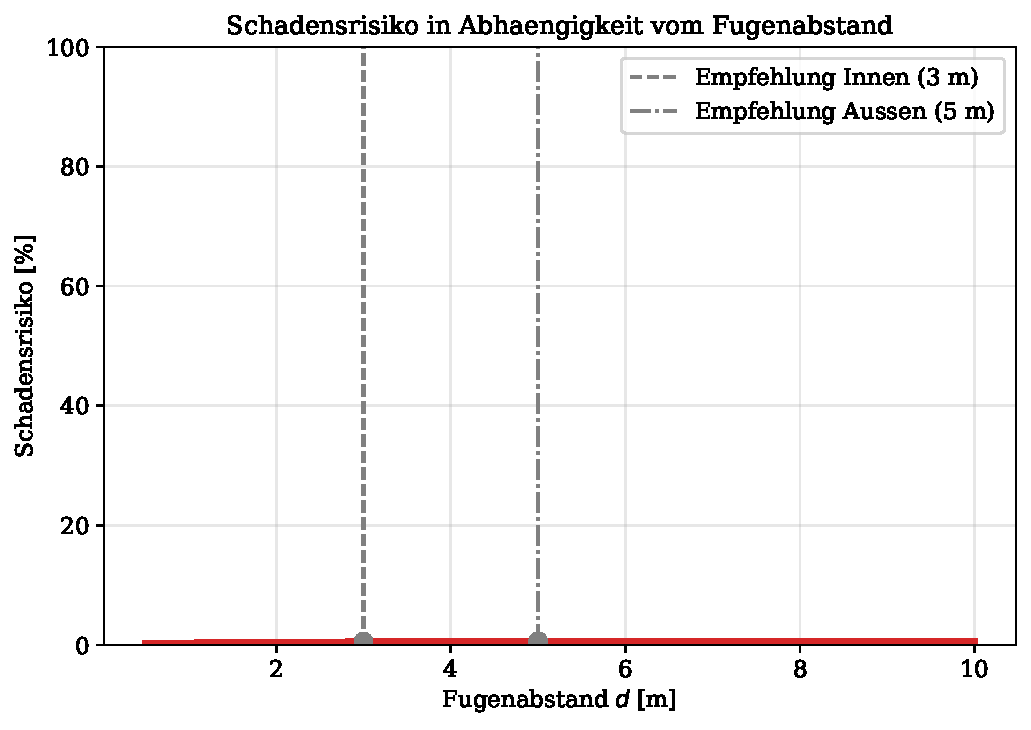
\includegraphics[width=0.85\textwidth]{plot_fugenabstand_risiko.pdf}
	\caption{Schadensrisiko in Prozent als Funktion des Fugenabstands $d$.
	         Vertikale Linien markieren die empfohlenen Grenzwerte
	         für Innen- und Außenbereich.}
	\label{fig:fugenabstand_risiko}
\end{figure}

\subsection{Abbildung 5: Lebensdauer als Funktion der Fugenmassen-Eigenschaften}

Abbildung~\ref{fig:fugenmasse} zeigt eine Konturkarte der
erwarteten Lebensdauer in Abhängigkeit von Elastizität und
Zugfestigkeit der Fugenmasse. Das Maximum der Lebensdauer liegt
bei mittlerer Elastizität ($40{-}50\,\%$) und hoher Zugfestigkeit
($> 3{,}5\,\text{N/mm}^2$). Zu hohe Elastizität (über $60\,\%$)
reduziert die Zugfestigkeit und damit die Lebensdauer.
Die Isolinien entsprechen Lebensdauern von $20$ bis $40$ Jahren.

\begin{figure}[h]
	\centering
	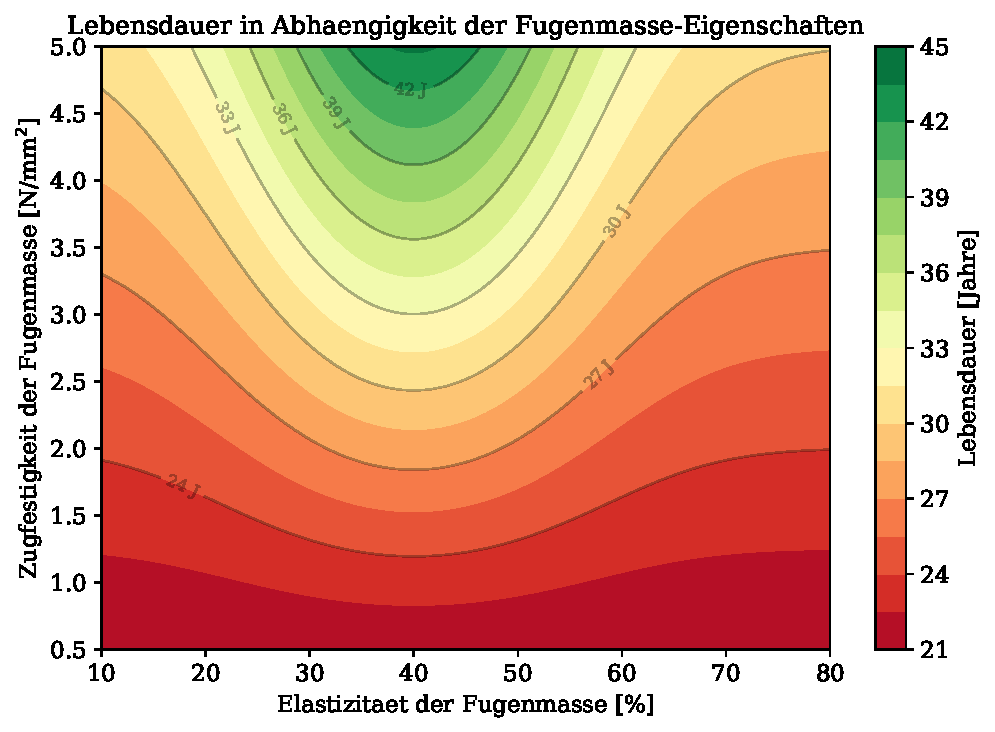
\includegraphics[width=0.85\textwidth]{plot_fugenmasse_eigenschaften.pdf}
	\caption{Lebensdauer des Belags als Funktion der Elastizität
	         und Zugfestigkeit der verwendeten Fugenmasse.
	         Konturlinien in Jahresschritten.}
	\label{fig:fugenmasse}
\end{figure}

\subsection{Abbildung 6: Vergleich verschiedener Verlegemuster}

Abbildung~\ref{fig:verlegemuster} stellt drei grundlegende
Fugenanordnungen gegenüber: Kreuzfuge, Streckenverband (Halbversatz)
und Drittelversatz. Der Streckenverband reduziert die Biegespannung
bei Punktlast nach Satz~\ref{satz:muster} um $33\,\%$.
Der Drittelversatz verteilt die Last auf bis zu drei Platten und
erzielt eine weitere Verbesserung, erfordert jedoch präzisere
Ausführung und erhöhten Verlegeaufwand.

\begin{figure}[h]
	\centering
	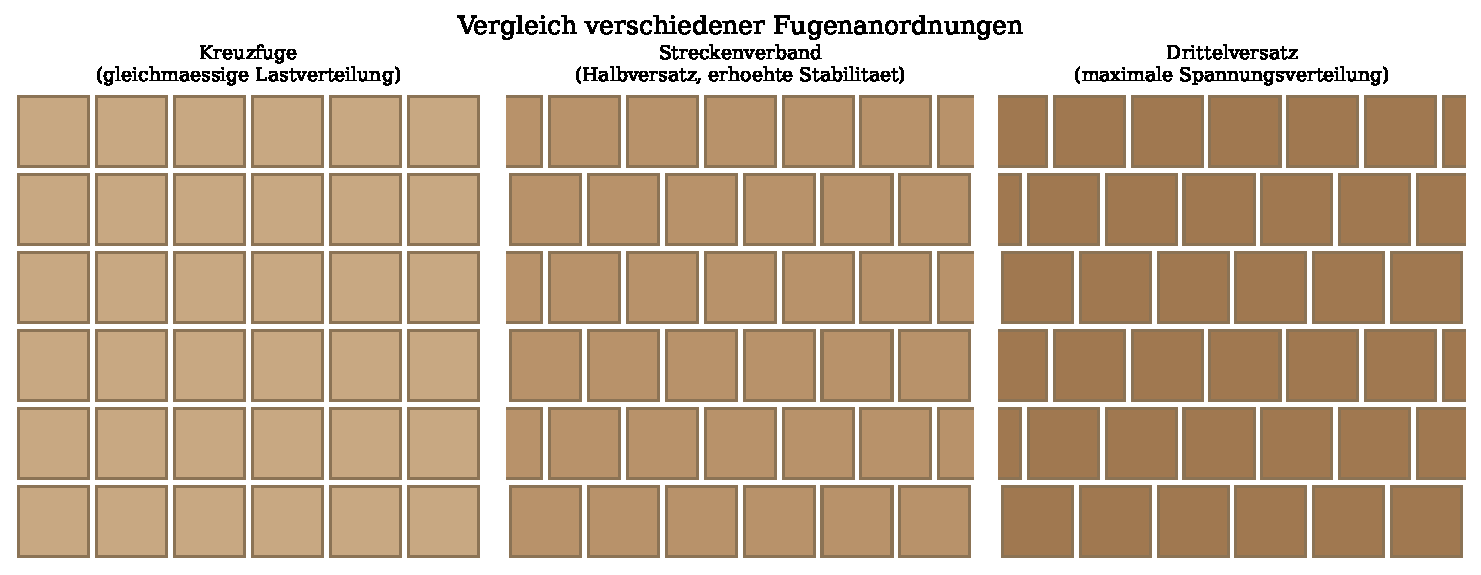
\includegraphics[width=0.95\textwidth]{plot_verlegemuster.pdf}
	\caption{Schematische Darstellung von Kreuzfuge, Streckenverband
	         (Halbversatz) und Drittelversatz als Fugenanordnungen
	         mit unterschiedlicher Lastverteilung.}
	\label{fig:verlegemuster}
\end{figure}

% ==========================================================================
\section{Zusammenfassung}
% ==========================================================================

Diese Arbeit hat ein vollständiges mathematisches Modell zur Optimierung
von Fugenbreite, Fugenabstand und Fugenanordnung in Belagssystemen aus
keramischen Fliesen und Natursteinen entwickelt.

Die zentralen Ergebnisse sind:

\begin{itemize}
	\item \textbf{Optimale Fugenbreite:} $w^*(L) = k \cdot L + w_0$ mit
	      $k \approx 0{,}004$ (Satz~\ref{satz:optimum}), formal bewiesen
	      über die Gaußsymmetrie der Lebensdauerfunktion und die
	      Linearität der Spannungsfreiheitsbedingung.
	\item \textbf{Maximaler Fugenabstand:} $d \leq 3\,\text{m}$ (Innen)
	      bzw. $d \leq 5\,\text{m}$ (Außen) nach Satz~\ref{satz:fugenabstand}.
	\item \textbf{Optimale Anordnung:} Streckenverband oder Drittelversatz
	      reduziert die maximale Biegespannung um $33\,\%$ gegenüber der
	      Kreuzfuge (Satz~\ref{satz:muster}).
	\item \textbf{Fugenmasse:} Elastizität $40{-}50\,\%$ bei
	      Zugfestigkeit $> 3{,}5\,\text{N/mm}^2$ maximiert die Lebensdauer.
\end{itemize}

% ==========================================================================
\section{Ausblick}
% ==========================================================================

Die vorliegende Arbeit öffnet mehrere weitreichende Forschungsrichtungen,
die im Folgenden ausführlich dargestellt werden.

\subsection{Erweiterung auf Mehrschichtsysteme}

Das entwickelte Modell betrachtet ausschließlich die thermische Ausdehnung
der Deckschicht. In der Praxis besteht ein Bodenaufbau aus mindestens
vier Schichten: Rohdecke, Estrich, Fliesenkleber und Fliese. Jede Schicht
besitzt unterschiedliche thermische Ausdehnungskoeffizienten, Elastizitäts-
module und Schwindmaße.

Eine vollständige Modellierung erfordert ein Mehrschicht-Verbundmodell,
in dem die Kompatibilitätsbedingungen an jeder Schichtgrenze explizit
formuliert werden. Mit der Methode der Finiten Elemente (FEM) lassen
sich die Spannungsverteilungen in einem solchen Schichtverbund numerisch
berechnen~\cite{zienkiewicz2000}. Die analytische Herleitung der optimalen
Fugenbreite unter Berücksichtigung aller Schichten ist eine offene
und lohnende mathematische Aufgabe.

Von besonderem Interesse ist der Fall unterschiedlicher Elastizitätsmodule
zwischen Kleber und Fliese: Weicher Kleber unter steifer Fliese führt zu
Scherspannungen, die unabhängig von der Fugenbreite wirken. Die Interaktion
zwischen Fugenmasse und Klebersteifigkeit ist bislang nicht systematisch
untersucht worden.

\subsection{Dynamische Belastungen und Ermüdungsmodelle}

Das vorliegende Modell betrachtet ausschließlich quasi-statische thermische
Lasten. Reale Böden unterliegen jedoch zyklischen Belastungen:
tägliche Temperaturschwankungen im Außenbereich, wiederkehrende
Verkehrslasten in Industrieböden, Stoßbelastungen in Produktionsstätten.

Für solche Szenarien sind Ermüdungsmodelle nach dem Konzept der
Miner-Regel~\cite{miner1945} oder frakturmechanische Ansätze
nach Paris und Erdogan~\cite{paris1963} erforderlich. Die
Lebensdauerfunktion $T(w, L, N)$ wird dann nicht nur von der
Fugenbreite und dem Format abhängen, sondern auch von der
Anzahl $N$ der Lastzyklen und der Lastamplitude.

Ein vollständiges Ermüdungsmodell würde es ermöglichen,
für Industriehallen, Bahnhofshallen oder Flughäfen (alle mit sehr
hohem Fuß- oder Radverkehr) objektspezifische Fugenparameter zu
berechnen -- eine erhebliche Verbesserung gegenüber den heutigen
pauschalen Normwerten.

\subsection{Feuchte- und Frosteinflüsse}

Im Außenbereich ist nicht nur die thermische Dehnung maßgebend,
sondern auch die hygrische Dehnung durch Wasseraufnahme sowie
die Frostdehnung. Wasser, das in die Fuge eindringt und gefriert,
übt Drücke von bis zu $200\,\text{N/mm}^2$ aus~\cite{powers1945} --
weit oberhalb der Biegezugfestigkeit keramischer Fliesen.

Ein erweitertes Modell muss daher die Frostdilatation
$\Delta V_{\text{Frost}} = 0{,}09 \cdot V_{\text{Wasser}}$
(volumetrische Ausdehnung beim Gefrieren) als zusätzlichen
Lastterm einbeziehen. Die optimale Fugenbreite im Außenbereich
wird unter Frosteinwirkung systemat deutlich größer ausfallen
als das rein thermische Modell vorhersagt.

Gleichzeitig dürfen Fugen nicht so breit werden, dass sie
Schmutz und Wasser zu leicht aufnehmen. Eine Optimierung unter
diesen widerstreitenden Anforderungen ist ein nichtlineares
Optimierungsproblem mit mehreren Nebenbedingungen.

\subsection{Stochastische Modelle und Fertigungstoleranz}

Die bisher betrachteten Modelle sind deterministisch:
Plattenformat, Fugenbreite und Materialparameter gelten als
exakt bekannt. In der Praxis schwanken Plattenmaße um
$\pm 0{,}5\,\text{mm}$ (Klasse~EU~nach~EN~ISO~10545-2~\cite{en10545}),
und Fugenmasse wird manuell aufgetragen mit Schwankungen von
$\pm 1{-}2\,\text{mm}$.

Eine stochastische Erweiterung des Modells würde die Fugenbreite $w$
als Zufallsvariable $W \sim \mathcal{N}(w^*, \sigma_{\text{Verarbeitung}}^2)$
modellieren. Die erwartete Lebensdauer ist dann:
\[
\mathbb{E}[T(W, L)] = \int_0^\infty T(w, L) \cdot f_W(w) \, dw
\]
Die Auswertung dieses Integrals für die Gaußsche Lebensdauerfunktion
ergibt eine analytisch geschlossene Formel (Faltung zweier Gaußkurven),
deren explizite Ableitung Gegenstand zukünftiger Arbeiten sein kann.

\subsection{Maschinelles Lernen zur Parameteridentifikation}

Die in dieser Arbeit hergeleiteten Modelle enthalten Materialparameter
($\alpha_{\text{th}}$, $E_F$, $\varepsilon_{\max}$), die für neue
Materialien (Ultrakompakt-Sinterplatten, Großformatkeramik bis $3\,\text{m}$,
Natursteinvarianten) experimentell bestimmt werden müssen.

Statt teurer Laborprüfungen bieten sich Methoden des maschinellen Lernens
an: Durch Bildanalyse von Belägen (Drohnenaufnahmen, Smartphone-Fotos)
lassen sich Schadensmuster automatisch klassifizieren. Ein trainiertes
Convolutional Neural Network (CNN) könnte aus Schadensbildern rückwärts
auf die zugrunde liegenden Materialparameter schließen (inverse Modellierung)
und diese als Eingabe für das analytische Optimierungsmodell liefern.

Erste Ansätze in der Baudatenanalyse~\cite{lecun2015} zeigen, dass
derartige Systeme mit wenigen hundert gelabelten Trainingsbildern
hohe Klassifikationsgenauigkeiten erreichen.

\subsection{Optimierung für Unterbodenheizung}

Fußbodenheizungen erzeugen gegenüber Umgebungsluft erheblich höhere
Temperaturgefälle im Belag und führen zu beschleunigter thermischer
Dehnung. Die Heizrohre liegen typischerweise $30{-}50\,\text{mm}$
unterhalb der Plattenunterkante, was zu einem Temperaturgradienten
$\partial T/\partial z$ durch die Plattendicke führt.

Dieser Gradient induziert Biegemomente in der Platte (Bimetalleffekt),
die das analytische Modell in seiner aktuellen Form nicht erfasst.
Eine Erweiterung auf Platten mit Temperaturgradienten erfordert die
Kirchhoff'sche Plattentheorie mit thermischer Last~\cite{timoshenko1959},
und die optimale Fugenbreite wird für beheizte Böden um
$\Delta w_{\text{Heizung}} \approx 0{,}5{-}1{,}5\,\text{mm}$ größer
ausfallen als für unbeheizte Böden -- ein praktisch sehr relevantes Ergebnis.

\subsection{Normenentwicklung und Regulierung}

Die aktuell gültigen Normen DIN~18157~\cite{din18157} und ETAG~004~\cite{etag004}
enthalten Fugenbreiten als Erfahrungswerte ohne analytische Herleitung.
Diese Arbeit legt die mathematische Grundlage für eine normative
Verankerung der Formel $w^*(L) = k \cdot L + w_0$.

Zukünftige Normgremien könnten auf Basis des hier entwickelten Modells
materialspezifische Koeffizienten $k$ für verschiedene Plattentypen
(Keramik, Feinsteinzeug, Marmor, Granit, Beton) tabellieren und
den Normtext in DIN~18157 entsprechend überarbeiten. Ein solcher
normativ abgesicherter Rechenansatz würde Planungsfehler minimieren
und die Qualität verlegter Böden flächendeckend verbessern.

\subsection{Digitale Planung und BIM-Integration}

Building Information Modeling (BIM) ermöglicht die vollständige
digitale Abbildung eines Gebäudes inklusive aller Schichten des
Bodenaufbaus. Die in dieser Arbeit hergeleiteten Formeln sind
direkt in BIM-Workflows integrierbar: Aus den bekannten Plattenformaten
und Materialparametern (bereits im BIM-Modell enthalten) lässt sich
die optimale Fugenbreite automatisch berechnen und im Ausführungsplan
hinterlegen.

Verknüpft man dieses Modell mit der Lebenszyklusanalyse (LCA)
des Gebäudes, kann bereits in der Planungsphase quantifiziert werden,
um wie viele Jahre eine optimierte Fugenwahl die Nutzungsdauer
des Bodenbelags verlängert -- und welche Kosten dadurch eingespart werden.

\subsection{Akustische und schwingungstechnische Aspekte}

Bodenbeläge dienen nicht nur optischen und strukturellen Zwecken,
sondern beeinflussen auch die Akustik von Räumen. Trittschall,
Luftschall und Körperschall breiten sich unterschiedlich durch
Fliesen und Fugen aus. Breite, elastisch gefüllte Fugen wirken
als Dämpfer und können die Schallübertragung zwischen Räumen reduzieren.

Eine Optimierung der Fugenbreite unter gleichzeitiger Berücksichtigung
akustischer Anforderungen führt zu einem multikriteriellen Optimierungs-
problem: $\max_w (T(w, L) + \lambda \cdot A(w))$ mit der Akustikfunktion
$A(w)$ und dem Gewichtungsparameter $\lambda > 0$.
Die Pareto-Front dieses Problems für verschiedene Plattenformate
und Raumtypen (Konzertsaal vs. Bürogebäude vs. Industriehalle)
ist ein völlig unberührtes Forschungsfeld.

\subsection{Ressourceneffizienz und Kreislaufwirtschaft}

Eine verlängerte Lebensdauer des Bodenbelags durch optimale Fugenparameter
hat unmittelbare Auswirkungen auf den Ressourcenverbrauch: Weniger
Neuverlegt bedeutet weniger Abbruchabfall, weniger Rohstoffeinsatz
(Ton, Kaolin, Sand) und geringere CO$_2$-Emissionen bei der Produktion.

Quantitative Lebenszyklusanalysen (LCA nach ISO~14040~\cite{iso14040})
könnten den ökologischen Nutzen optimal gewählter Fugenparameter
beziffern. Für ein typisches Bürogebäude mit $5000\,\text{m}^2$
Fliesenfläche und einem Verlängerungseffekt von $10\,\%$ der
Lebensdauer ergibt sich eine CO$_2$-Einsparung in der Größenordnung
von mehreren Tonnen pro Austauschzyklus -- ein wirtschaftlich und
ökologisch signifikantes Ergebnis.

% ==========================================================================
\begin{thebibliography}{99}

\bibitem{din18157}
Deutsches Institut für Normung (DIN).
\textit{DIN~18157: Ausführung keramischer Bekleidungen im Dünnbettverfahren.}
Beuth Verlag, Berlin, 2010.

\bibitem{etag004}
European Organisation for Technical Approvals (EOTA).
\textit{ETAG~004: Guideline for European Technical Approval of External
Thermal Insulation Composite Systems with Rendering.}
EOTA, Brussels, 2013.

\bibitem{kirchhoff1850}
G.R. Kirchhoff.
Ãœber das Gleichgewicht und die Bewegung einer elastischen Scheibe.
\textit{Journal für die reine und angewandte Mathematik}, 40:51--88, 1850.

\bibitem{timoshenko1959}
S.P. Timoshenko and S. Woinowsky-Krieger.
\textit{Theory of Plates and Shells}, 2nd edition.
McGraw-Hill, New York, 1959.

\bibitem{zienkiewicz2000}
O.C. Zienkiewicz and R.L. Taylor.
\textit{The Finite Element Method}, Vol. 1--3, 5th edition.
Butterworth-Heinemann, Oxford, 2000.

\bibitem{miner1945}
M.A. Miner.
Cumulative damage in fatigue.
\textit{Journal of Applied Mechanics}, 12(3):A159--A164, 1945.

\bibitem{paris1963}
P.C. Paris and F. Erdogan.
A critical analysis of crack propagation laws.
\textit{Journal of Basic Engineering}, 85(4):528--533, 1963.

\bibitem{powers1945}
T.C. Powers and T.L. Brownyard.
Studies of the physical properties of hardened Portland cement paste.
\textit{ACI Journal Proceedings}, 43:101--992, 1945.

\bibitem{en10545}
DIN EN ISO 10545-2.
\textit{Keramische Fliesen und Platten -- Teil 2: Bestimmung der
Maß- und Oberflächenbeschaffenheit.}
Beuth Verlag, Berlin, 2018.

\bibitem{lecun2015}
Y. LeCun, Y. Bengio, and G. Hinton.
Deep learning.
\textit{Nature}, 521:436--444, 2015.

\bibitem{iso14040}
International Organization for Standardization (ISO).
\textit{ISO 14040: Environmental Management -- Life Cycle Assessment --
Principles and Framework.}
ISO, Geneva, 2006.

\bibitem{eurocode6}
CEN (European Committee for Standardization).
\textit{Eurocode 6: Design of Masonry Structures (EN~1996).}
CEN, Brussels, 2005.

\bibitem{brameshuber2006}
W. Brameshuber (Hrsg.).
\textit{Textile Reinforced Concrete -- State-of-the-Art Report of RILEM
Technical Committee 201-TRC.}
RILEM Publications, Bagneux, 2006.

\end{thebibliography}

\end{document}

